\section{Experiments}

\subsection{Dataset}
Dataset and experiment desig.

\subsection{Experiment Setup}

\subsubsection{Algorithms}
We compared the results of our framework (\textbf{APART}) with two other approaches; \textbf{SP} (i.e., Shortest Path) and \textbf{NN} (i.e., Nearest Neighbor).

Our implementation of SP is based on the algorithms in \cite{Huang14}. The only advantage of \cite{Huang14} over \cite{Ma13} is the the former considers reordering of the schedule while the latter does not. Although it is shown the performance increase of reordering requests is minimal, since we consider request reordering in APART, we decided to base the SP implementation on algorithms in \cite{Huang14} to make the comparison as fair as possible. We incorporate the notion of monetary incentives similar to \cite{Ma15} such that we only assign the request to a driver if it satisfies the monetary constraints of all riders, otherwise we check the next driver with least increase in traveled distance.

Also, the NN algorithm is implemented based on the current approach adopted by major ridesharing platforms such as Uber. The NN approach, finds the first nearest driver to the pick-up location of a new request. If the driver is able to fit the new request in its schedule without violating any constraints, he accepts the request. Otherwise the request is rejected and the algorithm tries to assign the request to the next nearest driver. This continues until a driver accepts the request of every driver rejects it in which case the request is dropped.

As a result, we are comparing the performance of APART with state-of-the-art approaches from both academia (SP) and industry (NN).

In the first set of experiments, we use the pricing model explained in \cref{sec:pricing} and compare the three approaches. Later in \cref{subsec:pricingexp} we utilize the pricing model introduced in \cite{Ma15} for both APART and SP. In the pricing model of \cite{Ma15}, there is no concept of \textit{revenue} similar to what we introduced in \cref{sec:pricing}. Therefore, in order to compare the generated revenue, we assume each driver has to pay 20\% of what they make as the server's share.

\subsubsection{Configurations and Measures}
In our experiments we measure three different metrics by varying different parameters of the system. We measure (1) service rate as the percentage of requests that were completed, (2) the revenue of the system and (3) the response time for matching a request with a driver. Also, \cref{tab:params} shows the different values we used for various parameters to evaluate our framework (default values are shown in \textbf{bold}).

\TODO{mohammad}{Write default values for rider and driver profiles}

\begin{figure*}[]
    \centering
    \subfigure[\small{Service Rate}]{
        \label{fig:default_sr}
        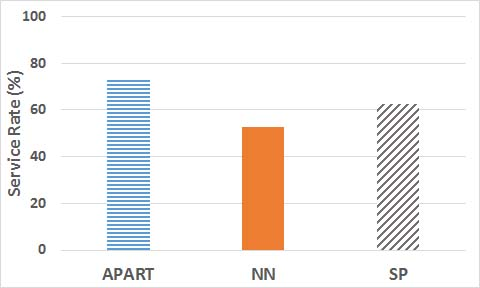
\includegraphics[width = 0.45\columnwidth]{fig/default_sr.jpg}
    }
    \subfigure[\small{Driver Availability}]{
        \label{fig:availability}
        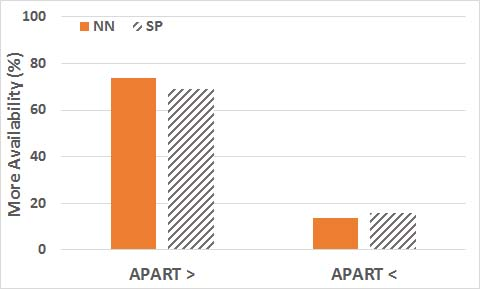
\includegraphics[width = 0.45\columnwidth]{fig/availability.jpg}
    }
    \subfigure[\small{Revenue}]{
        \label{fig:default_rev}
        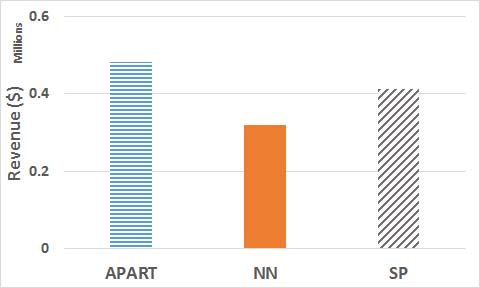
\includegraphics[width = 0.45\columnwidth]{fig/default_rev.jpg}
    }
    \subfigure[\small{Response Time}]{
        \label{fig:default_rp}
        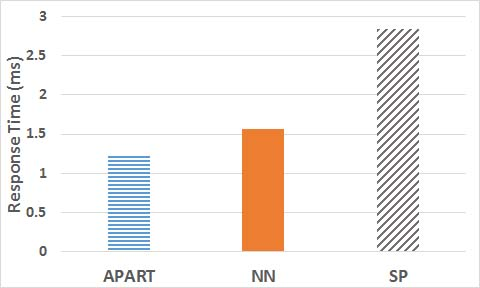
\includegraphics[width = 0.45\columnwidth]{fig/default_rp.jpg}
    }
    \vspace{-0.15in}
    \caption{Comparing Algorithms with Default Values}
    \label{fig:defaults}
\end{figure*}

\begin{table}
\begin{center}
\begin{tabular}{|c|c|}
	\hline
	Parameter & Values \\
	\hline \hline
	Max Wait Time & 3min, \textbf{6min}, 9min, 12min, 15min, 20min \\ 
	\hline
	\# of Drivers & 1000, 2000, \textbf{5000},  10000, 20000\\ 
	\hline
	Max Passengers & 2, 3, \textbf{4}, 5, 6 \\
	\hline
	Max Allowed Detour & 25\%, \textbf{50\%}, 75\%, 100\%\\
	\hline
\end{tabular}
\caption{Parameters for Algorithm Comparison}
\label{tab:params}
\end{center}
\end{table}

\subsection{Algorithm Comparison}
In this section, we compare and analyze the performance of the three approaches using the default parameters in \cref{tab:params}. The we evaluate the effect of different parameters by varying one of the parameters based on \cref{tab:params} while other parameters have their default values. We show how the algorithms compare to each other with regard to service rate, generated revenue and response time.

In \cref{fig:default_sr} we compare the service rate of the three algorithms. As it is shown, APART is able to serve more requests compared to the other two approaches. For all three approaches we use the same set of requests and drivers for each run. Than means all approaches start with the same configuration in the road network. However, each approach assigns riders to drivers differently and hence, after a while the dynamic of the network will be different in each algorithms. For each incoming request, we count the number of eligible workers (\cref{subsec:dispatch}). We say, the driver availability in algorithm $A$ is higher than $B$ with regard to request $r$, if during the simulation, in algorithm $A$ more eligible drivers are available for $r$ compared to algorithm $B$. \cref{fig:availability}, shows the percentage of the requests for which APART had higher(/lower) driver availability compared to the other two approaches. The left two bars in \cref{fig:availability} show that for more than 60\% of the requests, APART has a higher driver availability compared to both NN and SP. This means that APART engages drivers more effectively compared to NN and SP and hence, is able to serve more requests.

Next, we compare the algorithms with regard to how much revenue they generate. \cref{fig:default_rev} shows APART generate almost 20\% more revenue compared to SP and 50\% more than NN. Earlier we mentioned that the driver with minimum increase in his traveled distance is not necessarily the most profitable driver. To verify this theory, when running SP, for each incoming request, after the algorithm chose the driver with least increase in traveled distance, we also checked all eligible drivers to see which one generates the highest profit by serving the new request. We performed a similar check when running NN. According to the results for 23\% of the requests, the driver chosen by SP was different from the most profitable driver. This number for NN was 70\%. As we explained earlier, the implementation of SP and NN is such that the request does not get assigned to a driver that cannot satisfy the monetary constraint. In other words, both approaches make sure by assigning a request to a driver, the platform provider does not end up loosing money. If we removed this check in both approaches, in SP, 5\% of the requests would be assigned to drivers that would end up loosing money. For NN, this number would be 40\%.

The final metric we compared, was the average response time for processing a single request. As we see in \cref{fig:default_rp}, with the default setting, the processing time in SP is almost twice the response time in APART. The reason is that although SP utilizes the Kinetic Tree data structure in \cite{Huang14}, the server has to perform scheduling for eligible drivers sequentially while the auction-based approach in APART, distributes the scheduling to the drivers. Nevertheless, with the default settings, all three approaches process the requests under 3ms which is acceptable for a real-time framework.

Following we vary different parameters in the framework based on \cref{tab:params} and evaluate the effect of each parameter on the same metrics.

\subsubsection{Service Rate}
In these set of experiments we compare the service rate of the three approaches. As shown in \cref{fig:sr}, all algorithms generate high service rates when the constraints are loosened or there is high resource availability. However, under tight constraints or limited resources, APART outperform the other two approaches by up to 20\%. Earlier we showed how APART copes with the dynamism in the system better than the other two approaches.

\begin{figure}[h]
    \centering
    \subfigure[\small{Maximum Wait Time}]{
        \label{fig:mwt_sr}
        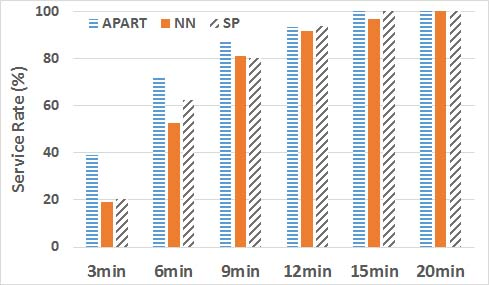
\includegraphics[width = 0.45\columnwidth]{fig/mwt_sr.jpg}
    }
    \subfigure[\small{Number of Drivers}]{
        \label{fig:nd_sr}
        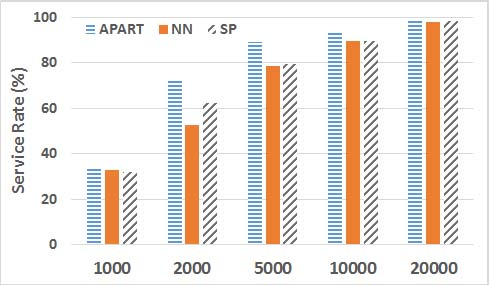
\includegraphics[width = 0.45\columnwidth]{fig/nd_sr.jpg}
    }
    \subfigure[\small{Maximum Passengers}]{
        \label{fig:mp_sr}
        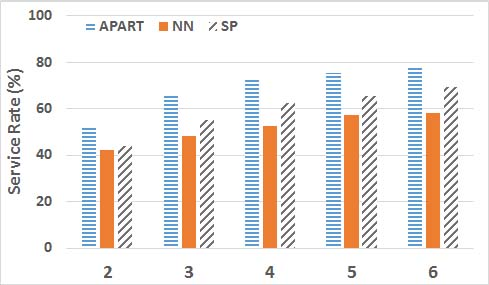
\includegraphics[width = 0.45\columnwidth]{fig/mp_sr.jpg}
    }
    \subfigure[\small{Maximum Allowed Detour}]{
        \label{fig:mad_sr}
        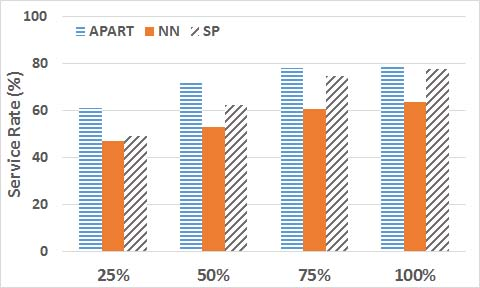
\includegraphics[width = 0.45\columnwidth]{fig/mad_sr.jpg}
    }
    \vspace{-0.15in}
    \caption{Comparing Service Rate of the Algorithms}
    \label{fig:sr}
\end{figure}

\subsubsection{Revenue}
As mentioned, the main objective of APART is to maximize the ridesharing platform's revenue. In these set of experiments, we compare the generated revenue of each algorithm. In these experiments we applied the pricing model explained in \cref{sec:pricing}. Here, we want to evaluate the effect of varying the parameters in \cref{tab:params} on the revenue and compare different algorithms. Later in \cref{subsec:pricingexp} we will apply different pricing models to the algorithms and compare revenue under different pricing models as well.

\begin{figure}[h]
    \centering
    \subfigure[\small{Maximum Wait Time}]{
        \label{fig:mwt_rev}
        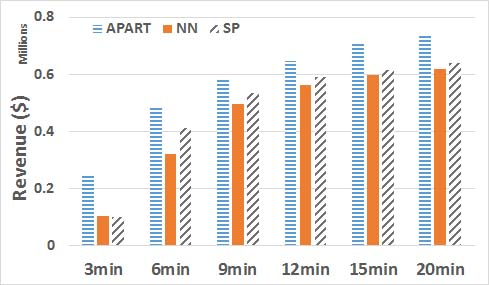
\includegraphics[width = 0.45\columnwidth]{fig/mwt_rev.jpg}
    }
    \subfigure[\small{Number of Drivers}]{
        \label{fig:nd_rev}
        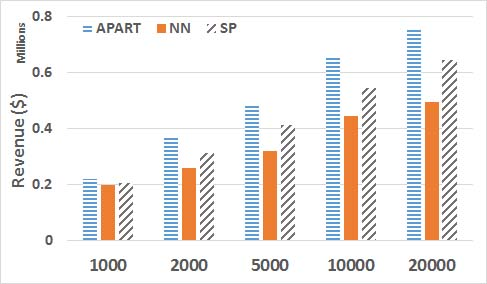
\includegraphics[width = 0.45\columnwidth]{fig/nd_rev.jpg}
    }
    \subfigure[\small{Maximum Passengers}]{
        \label{fig:mp_rev}
        \includegraphics[width = 0.45\columnwidth]{fig/mp_rev.jpg}
    }
    \subfigure[\small{Maximum Allowed Detour}]{
        \label{fig:mad_rev}
        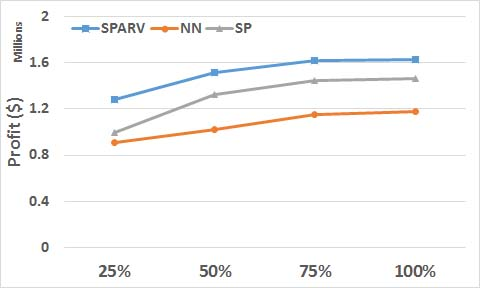
\includegraphics[width = 0.45\columnwidth]{fig/mad_rev.jpg}
    }
    \vspace{-0.15in}
    \caption{Comparing Revenue of the Algorithms}
    \label{fig:rev}
\end{figure}

As it can be seen in \cref{fig:rev} regardless of the values of different parameters, APART generates more revenue than any other approach. When we compare the results in \cref{fig:rev} with the ones in \cref{fig:sr}, even under configurations where all algorithms have the same service rate, APART manages to generate at least 10\% more revenue. The main reason for higher revenue is that APART is designed to make a \textit{Price-aware} assignment, i.e., assign the request to a driver that generates the most profit. Of course, as explained in \cref{sec:pricing}, the pricing models that are used in APART are designed such that the higher profits are not gained by scamming the riders. On the other hand, as it was explained earlier, the SP and NN algorithm were not designed to maximize revenue.

\subsubsection{Response Time}

Similar to \cite{Ma13,Huang14}, APART processes the requests, one request at a time once a request is submitted. In order to evaluate the scalability of our framework, our next set of experiments evaluate the response time of processing a single request. 

\begin{figure}[h]
    \centering
    \subfigure[\small{Maximum Wait Time}]{
        \label{fig:mwt_rp}
        \includegraphics[width = 0.45\columnwidth]{fig/mwt_rp.jpg}
    }
    \subfigure[\small{Number of Drivers}]{
        \label{fig:nd_rp}
        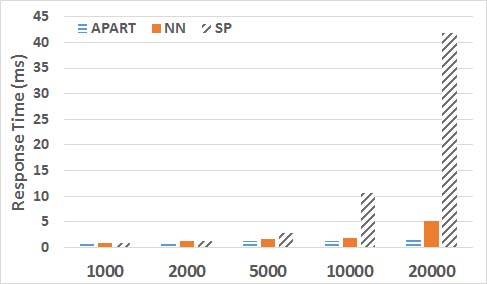
\includegraphics[width = 0.45\columnwidth]{fig/nd_rp.jpg}
    }
    \subfigure[\small{Maximum Passengers}]{
        \label{fig:mp_rp}
        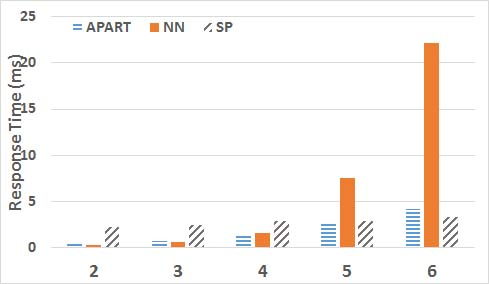
\includegraphics[width = 0.45\columnwidth]{fig/mp_rp.jpg}
    }
    \subfigure[\small{Maximum Allowed Detour}]{
        \label{fig:mad_rp}
        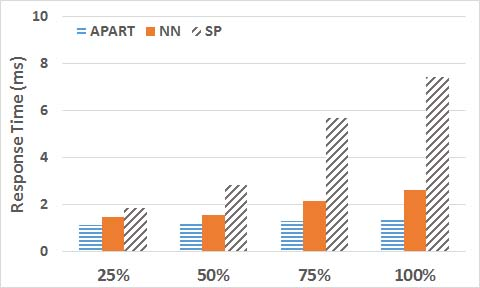
\includegraphics[width = 0.45\columnwidth]{fig/mad_rp.jpg}
    }
    \vspace{-0.15in}
    \caption{Comparing Revenue of the Algorithms}
    \label{fig:rp}
\end{figure}

In \cref{fig:nd_rp}, when more drivers are added, the scalability of SP suffers as it has to perform scheduling for a larger number of vehicles. On the other hand, due to the distributed nature of APART's auction-based approach, each driver does scheduling for itself and adding drivers does not affect the overall response time of APART as much. In \cref{fig:mp_rd} we notice that although APART's response time does not go beyond 5ms, SP handles the increase in maximum passengers better due to the Kinetic Tree structure implementation \cite{Huang14}. The reason for NN's poor performance in \cref{fig:mp_rp} is that it has to \textit{sequentially} perform a computation heavy scheduling, for possibly multiple drivers. Finally, in \cref{fig:mwt_rp} and \cref{fig:mad_rp} we notice that for loose constraints, the response time of SP increases up to 4 times higher than APART. The main reason is that the Kinetic Tree structure keeps track of all possible orders of requests that are assigned to a driver. As we loosen the constraints, the number of feasible permutations of the requests increases which makes the size of the Kinetic Tree larger and updates become computationally more expensive. This in turn increases the response time. \cref{fig:rp} shows unlike the other two approaches, APART's scalability does not suffer by varying different parameters on the framework.

\subsection{Comparing Pricing Models}
\label{subsec:pricingexp}

In this section, we evaluate the effect of the pricing model. First we show the importance of designing a fair pricing model. We utilize the three aproaches with the model in \cite{Ma13} and show how some riders may end up suffering by participating in ride-sharing. Subsequently, we perform some experiments on the model in \cite{Ma15} and show that as a result of price-aware assignments, regardless of the model, APART generates more revenue for the platform provider. At the end, we show the flexibility that the notion of profiles provides for the users of APART. 

\cref{fig:fairness} shows the result of utilizing the pricing model in \cite{Ma13}. Based on their pricing model, the driver's income is: $c.d_1 + (1+\alpha).c.d_2$ where $d_1$ is the distance the driver had only one rider on-board, $d_2$ is the total distance the driver had more than one rider on-board and $c$ is some predefined constant. $\alpha$ takes a value between 0 and 1 which determines the increase in the driver's income for serving more than one rider. As we see in \cref{fig:saved}, by participating in ride-sharing, the majority of riders save money (pay less as compared to riding alone). \cref{fig:saved} supports the claim in \cite{Ma13} that on average riders will end up saving money. However, \cref{fig:lost} shows that regardless of what algorithm is used, up to 10\% of riders end up paying more by participating in ride-sharing which is not acceptable. 

\begin{figure}[h!]
	\centering
    \subfigure[\small{Rider's that Saved Money}]{
        \label{fig:saved}
        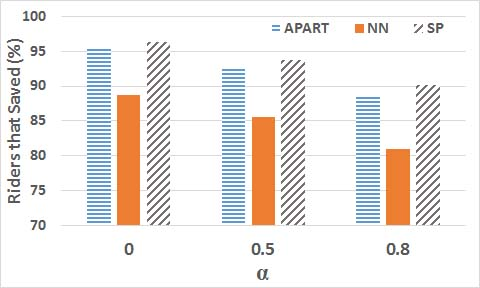
\includegraphics[width = 0.45\columnwidth]{fig/saved.jpg}
    }
    \subfigure[\small{Rider's that Lost Money}]{
        \label{fig:lost}
        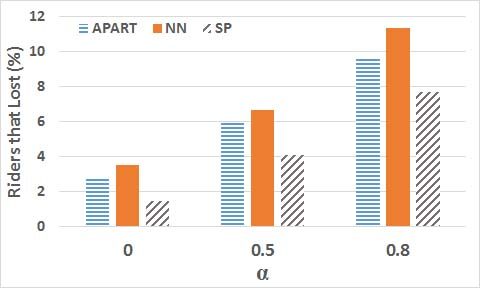
\includegraphics[width = 0.45\columnwidth]{fig/lost.jpg}
    }
    \vspace{-0.15in}
    \caption{Fairness of Pricing Models}
    \label{fig:fairness}
\end{figure}

In the next set of our experiments, we apply the model in \cite{Ma15} and evaluate the performance of APART and SP. In this model, riders get compensated for any detour incurred in their trip. The amount of compensation is based on the new rider's fare and the length of a rider's detour compared the the detour of other riders on the vehicle. \cref{fig:tkde_sr} shows that APART provides a slightly higher service rate than SP. However, due to assigning the riders to most profitable drivers, APART ends up generating 10\% more revenue.

\begin{figure}[h]
	\centering
    \subfigure[\small{Service Rate}]{
        \label{fig:tkde_sr}
        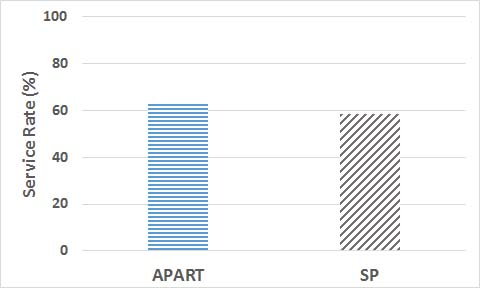
\includegraphics[width = 0.45\columnwidth]{fig/tkde_sr.jpg}
    }
    \subfigure[\small{Revenue}]{
        \label{fig:tkde_rev}
        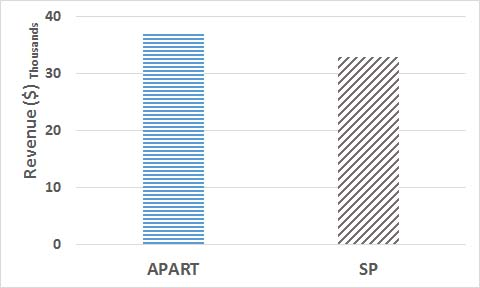
\includegraphics[width = 0.45\columnwidth]{fig/tkde_rev.jpg}
    }
    \vspace{-0.15in}
    \caption{Effect of Applying an Arbitrary Pricing Model}
    \label{fig:tkde}
\end{figure}

In \cref{sec:pricing} we mentioned by setting their profiles, users can configure APART to make assignments the way they find desirable. In the last set of our experiments, we used two different configurations for the riders' profiles. First, we set the riders' profiles to $f_T(\delta d_r) = \frac{1}{(\delta d_r + 1)}$. Such profile is suitable for a rider who wants to minimize his detour and is willing to share a ride only if the detour is short. Since the rider is setting \textbf{Tight} constraints we show this profile by $f_T$. In the second run, we set the profile of the riders to $f_R(\delta d_r) = 1 -  (\frac{\delta d_r}{max \delta})$. This profile is more \textbf{Relaxed} (hence, $f_R$) and it is expected that more riders share a trip. \cref{fig:quality} shows the result of utilizing APART and SP with $f_T$ and $f_R$. Since SP does not make price-aware assignments, the results in both runs were the same. However, as we can see with APART\_T, almost 10\% fewer riders ended up sharing a ride while on average they only observed 6-7\% increase in their trips. On the other hand, with APART\_R, almost every rider ended up sharing a ride and the average increase in their trip was almost 20\%. An interesting observation in \cref{fig:quality} is that with APART\_R, more riders ended up sharing a ride compared to SP while their average detour was still less.

\begin{figure}[h]
	\centering
    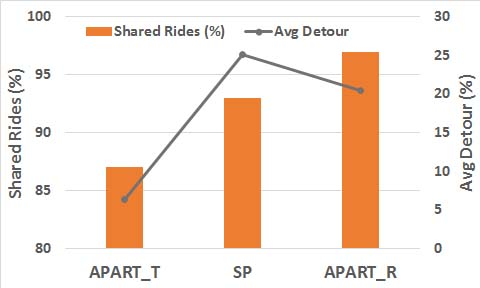
\includegraphics[width = 0.45\columnwidth]{fig/quality.jpg}
    \vspace{-0.15in}
    \caption{Effect of Profiles}
    \label{fig:quality}
\end{figure}

